\documentclass[8.01x]{subfiles}
\begin{document}

\chapter{Week 3: Homework 3}

\section{Problem 1: A block on a frictionless ramp}

\begin{center}
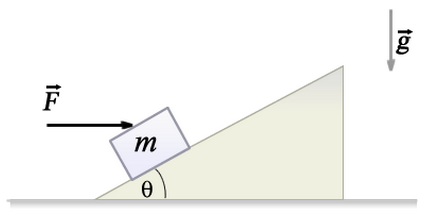
\includegraphics[scale=0.65]{Graphics/h3p1}
\end{center}

``A block of mass m = 4 kg is pressed with a horizontal force F against a frictionless ramp of angle $\theta = \ang{38}$.

Assuming the block is at rest on the ramp, answer the following:\\
(a) What is the magnitude of the normal force exerted by the incline surface on the block?\\
(b) What is the magnitude of the force F exerted on the block?''

We should start out by drawing a free-body diagram, but even before we do that, we need to decide on a coordinate system. I'm not sure if it'd be best to choose one where $y$ is perpendicular to the incline, or where it is parallel with $\vec{g}$. In either case, there are things we need to decompose; I'll therefore choose one where $+x$ is in the uphill direction, and $+y$ is perpendicular to the incline, so ``diagonally upwards'' in this case.

The forces we need to worry about are $\vec{F}$, $m \vec{g}$, and the normal force $\vec{N}$. Let's consider them together in the $x$ direction. The object is at rest, so via Newton's second law, the net force is zero.

\begin{equation}
F \cos \theta = m g sin \theta
\end{equation}

The normal force is perpendicular to the incline, and so the $x$ component is zero. Meanwhile, the $x$ component of the force $F$ applied must balance out the gravitational force $m g \sin \theta$ in the $x$ direction.

It's always a good idea to test the extremes and ensure the correct trig functions are used. If $\theta = 0$, we expect there to be no gravitational force at all in the $x$ direction, and indeed $\sin(0) = 0$. Using the same argument, if $\theta = 90$, the gravitational force should be exclusively in the $x$ direction, and again, it will be. As for $F \cos \theta$, the opposite is true, as it should be.

So far, so good. Next, let's look at the $y$ direction. Newton's second law, again:

\begin{align}
N = m g \cos \theta + F_y\\
N = m g \cos \theta + F \sin \theta
\end{align}

The normal force must balance out the gravitational force (angled) downwards, plus the $y$ component of the force $F$, which is also in the $-y$ direction (that becomes easier to see if $\theta$ is increased).

We now have two equations, and two unknowns ($F$ and $N$). Let's write the equations with the numbers substituted, and solve:

\begin{align}
F \cos(\ang{38}) &= (\SI{4}{kg})(\SI{9.8}{m/s^2}) \sin(\ang{38})\\
N &= (\SI{4}{kg})(\SI{9.8}{m/s^2}) \cos(\ang{38}) + F \sin(\ang{38})
\end{align}

The second equation alone gives us

\begin{equation}
N = (\SI{4}{kg})(\SI{9.8}{m/s^2}) \cos(\ang{38}) + F \sin(\ang{38}) \approx \SI{30.89}{N} + 0.6156 F
\end{equation}

And the first alone tells us

\begin{equation}
F = \frac{(\SI{4}{kg})(\SI{9.8}{m/s^2}) \sin(\ang{38})}{\cos(\ang{38})} = \SI{39.2}{N} \tan(\ang{38}) = \SI{30.63}{N}
\end{equation}

So the answer for (b) is \SI{30.63}{N}, while the first one is \SI{49.75}{N}.

\section{Problem 2: Towing a sled}

``A mother tows her daughter on a sled on level ice. The friction between the sled and the ice is negligible, and the tow rope makes an angle of $\theta$ to the horizontal. The combined mass of the sled and the child is $M$. The sled has an acceleration in the horizontal direction of magnitude $a$.

\begin{center}
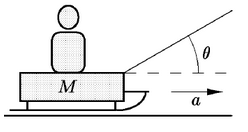
\includegraphics[scale=0.65]{Graphics/h3p2}
\end{center}

(a) Calculate the tension, $T$, in the rope. Express your answer in terms of $M$, $a$, $g$, and $\theta$.\\
(b) Calculate the magnitude of the normal force, $N$, exerted by the ice on the sled. Express your answer in terms of $M$, $a$, $g$, and $\theta$.''

First, let's identify the forces involved. There's the gravitational force $m g$ downwards, the normal force $N$ straight upwards, and the force from the rope, which will need some decomposition. Because of this, we can't simply state that $|N| = M g$; the rope is pulling upwards a bit, too.

Since there's no incline involved (for the sled itself), I choose a simple coordinate system where $+x$ is to the right, and $+y$ is straight upwards. The gravitational force is $-M g$, purely in the $y$ direction, and the acceleration is $a > 0$.\\
We can also express that in terms of a force $\displaystyle F_x = M a$, but let's be careful: this is not the force that the mother exerts; that force is at an angle $\theta$, so $F_x = F_{mother} \cos \theta$.

Writing Newton's second law for each of the two axes independently:

\begin{align}
F_x = M a\\
N + F_y = M g
\end{align}

We know that $F_x = F_{mother} \cos \theta$, so we can solve for $F_{mother}$ in terms of the acceleration and mass:

\begin{align}
F_{mother} = \frac{F_x}{\cos \theta} = \frac{M a}{\cos \theta}
\end{align}

How does this force relate to the tension $T$ in the rope, that we want to find out? It's actually not specified, but I assume we are to take the rope to be massless and of fixed length, as previously; especially as no mass is shown for the rope (nor is its length, by the way). Because of that, we can ignore the gravitational force on the rope.\\
So, long story short, $T = F_{mother}$, and we've already found the answer!

Next up, (b): $F_y = T \sin \theta$, so the third law equation becomes

\begin{equation}
N = M g - T \sin \theta
\end{equation}

If we substitute in the value for $T = F_{mother}$, we find

\begin{equation}
N = M g - \frac{M a \sin \theta}{\cos \theta} = M(g - a \tan \theta)
\end{equation}

... and we are done.

\section{Problem 3: Stacked blocks}

\begin{center}
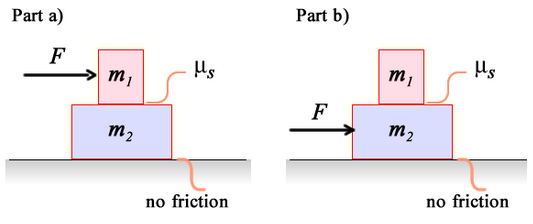
\includegraphics[scale=0.65]{Graphics/h3p3}
\end{center}

``Consider two blocks that are resting one on top of the other. The lower block has mass $m_2 = \SI{4.3}{kg}$ and is resting on a frictionless table. The upper block has mass $m_1 = \SI{1.2}{kg}$. Suppose the coefficient of static friction between the two blocks is given by $\mu_s = 0.6$.

Part a) A force of magnitude $F$ is applied as shown in the left figure above. What is the maximum force for which the upper block can be pushed horizontally so that the two blocks move together without slipping?''

As usual, let's start by looking at the forces involved. In the vertical direction, we have gravitational forces $g m_1$ and $g m_2$ acting on each of the blocks, respectively.\\
Block $m_1$ (or block 1) pushes downwards on block $m_2$ (or block 2) with that same force $g m_1$, and via Newton's third law, we find the reaction force (the normal force, in this case) from block 2 to block 1.

The total forces on block 1 are the gravitational force downwards, and the normal force upwards, from block 2 to 1. Net force: zero -- as it must be, since it is at rest.

As for block 2, the downward forces are as mentioned above $g m_1$ from the upper block, and $g m_2$ from gravity on the block itself. This is cancelled out by a normal force from the ground on the block, of magnitude $g(m_1 + m_2)$\footnote{Calculating like this may be a bad idea. I'll try to re-think for next time, and always consider one block at a time.}. Again, the net force is zero, at it must be.

With the normal force on block 1, we know that the maximum frictional force that will oppose motion in mass $m_1$ is $\mu_s N = \mu_s g m_1$. As for block 2, there is no friction to the ground, so we need not worry about the maximum frictional force there.

If we write a second law equation for mass $m_1$ on its own, and one for the entire system, both exclusively in the $x$ direction:

\begin{align}
F - F_{Fmax} &= m_1 a \text{ (top block)}\\
F &= a(m_1 + m_2) \text{ (entire system)}
\end{align}

The acceleration $a$ as seen from an external reference frame is equal for both, since the condition is that they move together. We can solve the second equation for $a$, and stick it into the first, and then solve for $F$:

\begin{align}
F - F_{Fmax} = m_1 \frac{F}{m_1 + m_2}\\
F - F \frac{m_1}{m_1 + m_2} = F_{Fmax}\\
F\left(1 - \frac{m_1}{m_1 + m_2}\right) = F_{Fmax}\\
F = \frac{F_{Fmax}}{1 - \frac{m_1}{m_1 + m_2}} = \frac{\mu_s g m_1}{1 - \frac{m_1}{m_1 + m_2}} \approx \SI{9.03}{N}
\end{align}

``Part b) A force of magnitude $F$ as shown in the right figure above. What is the maximum force for which the lower block can be pushed horizontally so that the two blocks move together without slipping?''

Okay, so we need to reverse the situation a bit. Except for the second law equations and such from above which clearly change, what else changes? The vertical forces don't; the maximum frictional force also doesn't, as it's based on the normal force, which is unchanged.\\
So, the force is now on $m_2$.

It seems like all we need to do is write a new pair of second law equations, again in the $x$ direction only. One equation remains unchanged, the one for the entire system. However, $F$ no longer acts on $m_1$!\\
Instead, it holds on via the frictional force, and can only accelerate together as long as that is ``strong'' enough.

If we push the lower block towards the right with too much force, what will happen? The upper block will glide ``backwards'', relative to the lower block. That means that the frictional force is now in the forward direction! Indeed, it's the only force acting on $m_1$ (horizontally), so we find

\begin{align}
F_{Fmax} = m_1 a \text{ (top block)}\\
F = a(m_1 + m_2) \text{ (entire system)}
\end{align}

Solving the first equation for $a$ and substituting into the second:
\begin{align}
F &= \frac{F_{Fmax}}{m_1}(m_1 + m_2)\\
  &= \frac{\mu_s g m_1}{m_1}(m_1 + m_2)\\
  &= \mu_s g(m_1 + m_2)
\end{align}

That's the second and final answer!

\section{Problem 4: Tension in string}

\begin{center}
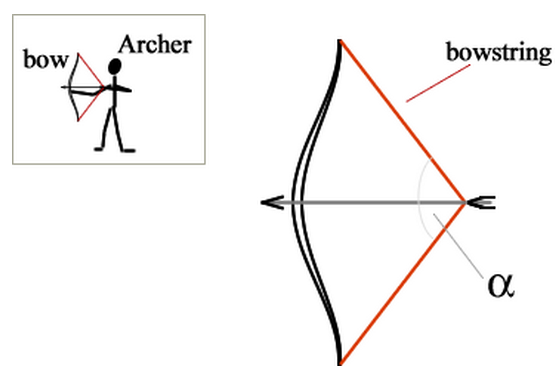
\includegraphics[scale=0.5]{Graphics/h3p4}
\end{center}

``An archer is preparing to shoot an arrow. He grabs the center of the bowstring and pulls straight back with a force of magnitude $F = 118$ N. The upper and lower halves of the string form an angle $\alpha = \ang{124}$ with respect to each other. Assume that the bowstring is massless.

(a) What is the magnitude of the tension in the upper half of the bowstring?''

Because the string is massless, we ignore the pull of gravity. That makes this the first problem of this week not to feature $g$ at all!	

Instead, because the string is at rest when he's done (I assume that's what they mean: he pulls the string backs, and then hold it in place such that $\alpha = \ang{124}$), the tension must balance his force out exactly, so that $a = 0$.

Let's choose a coordinate system where the archer pulls the string in the $+x$ direction (towards the right), and $+y$ is straight upwards. We call his force $F = (\SI{118}{N}) \hat{x}$. Any $y$ components in the tension must cancel each other out, and the $x$ components will cancel out with $F$.\\
Let's call the two tensions $T_U$ for upper, and $T_L$ for lower; each then have $x$ and $y$ components.

Because the archer pulls the rope towards the right, the tension points ``upwards to the left'' and `downward to the left'' in the upper and lower part of the string, respectively.

Decomposing the tension vectors, we find

\begin{align}
T_{Lx} &= T_L \cos (-\alpha/2)\\
T_{Ly} &= T_L \sin (-\alpha/2)\\
T_{Ux} &= T_U \cos (\alpha/2)\\
T_{Uy} &= T_U \sin (\alpha/2)
\end{align}

Writing Newton's second law for the archer's force ($+x$) and the tension forces ($-x$):

\begin{align}
F &= T_{Lx} + T_{Ux}\\
F &= T_L \cos (-\alpha/2) + T_U \cos (\alpha/2)
\end{align}

One equations, two unknowns. We can also write a second law equation for the vertical components of the tension, which will cancel:

\begin{align}
T_{Ly} &= -T_{Uy}\\
T_L \sin (-\alpha/2) &= -T_U \sin (\alpha/2)\\
T_L \sin (\alpha/2) &= T_U \sin (\alpha/2)\\
T_L &= T_U
\end{align}

The second-to-last step is because $\sin(-x) = -sin(x)$, so the minus signs cancel, and so we find that the tension is equal (in magnitude) for both parts of the string. With that in mind, we can write the other equation in terms of $T_L$ alone, and solve for it. Also, $\cos(-x) = \cos(x)$, so we can get rid of the duplicate cosine terms:

\begin{align}
F &= T_L \cos (-\alpha/2) + T_L \cos (\alpha/2)\\
F &= T_L (2\cos (\alpha/2))\\
T_L = T_U &= \frac{F}{2\cos (\alpha/2)} \approx \SI{125.67}{N}
\end{align}

And we are done!

\section{Problem 5: Measurement of friction coefficient}

``In Lecture 8 Video Segment 5, Prof. Lewin does two different experiments to calculate the coefficient of static friction of an inclined plane.

Experiment 1 took a measurement of the critical angle $\theta_c$ at which the block began to slide down the plane. Prof. Lewin measured the angle $\theta_c = \ang{20} \pm \ang{2}$.

Experiment 2 took a measurement of the critical mass $m_2$ which caused the block to begin to slide up the plane. Prof. Lewin measured the angle $\theta = \ang{20}$, the mass $m_1 = \SI{361(1)}{g}$, and the mass $m_2 = \SI{270(25)}{g}$.

For each of the following questions use only the uncertainties given above. Enter your answer to 3 or 4 significant figures to make sure it is within the grader's tolerance. take the value of $g$ to be $\SI{9.81}{m/s^2}$.

(a) What is the upper bound of the coefficient of static friction calculated from the data in Experiment 1?\\
(b) What is the lower bound of the coefficient of static friction calculated from the data in Experiment 1?''

Okay, so this first part should be easy. We found in lecture that $\mu_s = \tan \alpha$, only we call the angle $\theta_c$ here. The bounds are then found by taking the tangent of $\ang{18}$ and $\ang{22}$, and we're done: that gives us two values of $\mu_s$, one larger than the other; the larger is obviously the upper bound, then.

\begin{align}
\mu_{s_{max}} = \tan(\ang{22}) \approx 0.4040\\
\mu_{s_{min}} = \tan(\ang{18}) \approx 0.3249
\end{align}

We then move on to the second part, which is no doubt more work:

``(c) What is the upper bound of the coefficient of static friction calculated from the data in Experiment 2?\\
(d) What is the lower bound of the coefficient of static friction calculated from the data in Experiment 2?''

Okay. We know from the video that it's just about to go uphill. The condition that holds at that point is

\begin{align}
m_2 g &= m_1 g \sin \alpha + F_{Fmax}\\
m_2 g &= m_1 g \sin \alpha + \mu_s m_1 g \cos \alpha
\end{align}

$F_{Fmax}$ is given by $\mu_s N$, where $N$ is the normal force, $m_1 g \cos \alpha$. All of these equations are found in the video, and derived in that lecture (which I took notes of), so I won't repeat that. Let's try to solve this equation for $\mu_s$.

\begin{align}
m_2 g &= m_1 g \sin \alpha + \mu_s m_1 g \cos \alpha\\
\frac{m_2}{m_1} &= \sin \alpha + \mu_s \cos \alpha\\
\frac{m_2}{m_1} - \sin \alpha &= \mu_s \cos \alpha\\
\frac{\frac{m_2}{m_1} - \sin \alpha}{\cos \alpha} &= \mu_s\\
\frac{m_2}{m_1 \cos \alpha} - \tan \alpha &= \mu_s
\end{align}

Ah, not too bad. Now, for this part of the problem, $\theta = \ang{20}$ exactly, with no uncertainty given, while the masses have an uncertainty. It should be easy to find the upper bound: maximize $m_2$, and minimize $m_1$. For the lower bound, we do the opposite. Easy!

\begin{align}
\mu_{s_{max}} = \frac{\SI{295}{g}}{(\SI{360}{g}) \cos(\ang{20})} - \tan(\ang{20}) = 0.5081\\
\mu_{s_{min}} = \frac{\SI{245}{g}}{(\SI{362}{g}) \cos(\ang{20})} - \tan(\ang{20}) = 0.3563\\
\end{align}

Both answers (or all four, I suppose) are marked as correct. Excellent!\\
The ranges don't quite agree with each other, but there is indeed a range where the friction coefficient could be equal: 0.3563 - 0.4040 is allowed by both experiments.

\section{Problem 6: Rope between trees}

``Suppose a rope of mass m hangs between two trees. The ends of the rope are at the same height and they make an angle $\theta$ with the trees.

\begin{center}
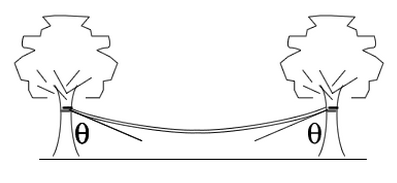
\includegraphics[scale=0.5]{Graphics/h3p6}
\end{center}

(a) What is the tension at the ends of the rope where it is connected to the trees? Express your answer in terms of $m$, $g$, and $\theta$.''

First off, note that $\theta$ is measured with respect to the \emph{vertical}, not the horizontal! If $\theta \approx \ang{90}$ then the rope is almost horizontal! In the figure above, I would estimate it around $\theta \approx \ang{70}-\ang{80}$ or something.

Now... For this first part, we can assume that all the mass of the rope is located at the exact middle, and we will find the same result for the tension at the trees (but clearly we can't use this method in part b).

We can therefore apply the same method Prof. Lewin used in a problem solving video. I don't recall it exactly, and I will try to re-derive it instead of re-watching, since my goal is to learn, not just to get a green checkmark! First off, he simplified the rope by drawing it as two straight lines, meeting at a large angle in the middle. If we then draw a dotted line horizontally between the points where the rope attaches, we get an obtuse triangle. I'll call the two side angles $\alpha$ (they are clearly equal), and the bottom, obtuse angle $\beta$. From the diagram, it's clear that

\begin{align}
\theta + \alpha = \ang{90}\\
\alpha = \ang{90} - \theta
\end{align}

With that in mind, plus the fact that $2 \alpha + \beta = \ang{180}$, we find $\beta = 180 - 2(90 - \theta) = 2 \theta$.

Okay, so having all that done, let's  look at some forces. At the exact center, there is a downwards force $m g$ due to gravity, which must be exactly balanced out. Only the $y$ component of the string tension could possibly counter this, so $T_y = m g$ (Newton's second law, relating only magnitudes) must hold, or there would be acceleration.

What is $T_y$, then? By some vector decomposition, it must be

\begin{equation}
T_y = T \sin \alpha
\end{equation}

... since $T_y$ is opposite the angle, while $T$ is the hypotenuse. We put this into the second law equation:

\begin{align}
T \sin \alpha &= m g\\
T &= \frac{m g}{\sin \alpha}\\
T &= \frac{m g}{\sin (\ang{90} - \theta)}\\
T &= \frac{m g}{\cos\theta}
\end{align}

What exactly is $T$, though? It's not the answer for either question -- we are not quite done yet. Instead, this is the total tension (or total force) the trees need to carry. Since there is symmetry in the problem, each tree carries \emph{half} this weight, which makes the answer for (a)

\begin{equation}
T_{tree} = \frac{m g}{2 \cos \theta}
\end{equation}

To find the next part, we need to use some symmetry.At the \emph{exact} center, which is mostly a theoretical concept, there is a point that has no weight. It has an infinitely small size, and it doesn't need to ``carry'' any other part of the rope, either. Therefore, the vertical component of the tension is zero, and only the horizontal component of the tension remains. Therefore, we take the horizontal component of the above: $T_x = T \cos \alpha = T \sin \theta$

\begin{align}
T_{middle} = \frac{m g}{2 \cos \theta} \sin \theta = \frac{m g}{2} \tan \theta
\end{align}

\section{Problem 7: Blocks and ramp with friction}

``A block of mass $m_1 = \SI{28}{kg}$ rests on a wedge of angle $\theta = \ang{47}$ which is itself attached to a table (the wedge does not move in this problem). An inextensible string is attached to $m_1$, passes over a frictionless pulley at the top of the wedge, and is then attached to another block of mass $m_2 = \SI{3}{kg}$. The coefficient of kinetic friction between block 1 and the plane is $\mu = 0.8$. The string and wedge are long enough to ensure neither block hits the pulley or the table in this problem, and you may assume that block 1 never reaches the table. Take $g$ to be \SI{9.81}{m/s^2}.

\begin{center}
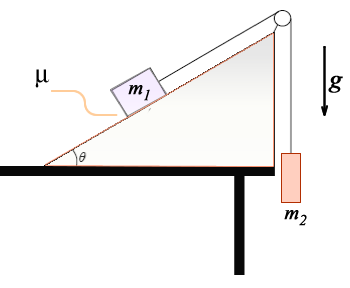
\includegraphics[scale=0.7]{Graphics/h3p7}
\end{center}

The system is released from rest as shown above, at $t = 0$.\\
(a) Find the magnitude of the acceleration of block 1 when it is released (in $\text{ m/s}^2$).''

Since $m_1$ is much greater than $m_2$, plus the fact that they only give us the \emph{kinetic} friction coefficient, along with ``and you may assume that block 1 never reaches the table'', I think it's quite safe to assume the system will accelerate ``counterclockwise'', so that $m_1$ slides down towards the table.

If we draw up a free-body diagram, we find the following forces acting on block $m_1$, assuming a coordinate system where $+x$ is downhill and $+y$ is perpendicular to the surface (diagonally upwards to the left):

\begin{itemize}
\item $m_1 g \cos \theta$ acting in the $-y$ direction
\item $N = m_1 g \cos \theta$ acting in the $+y$ direction, to cancel out the gravitational force
\item $m_1 g \sin \theta$ acting in the $+x$ direction
\item $F_f = \mu N = \mu m_1 g \cos \theta$ acting in the $-x$ direction
\item $T$ (unknown magnitude) acting in the $-x$ direction
\end{itemize}

As for the mass $m_2$, there are only two forces:

\begin{itemize}
\item $m_2 g$ acting downwards (which we call $-y$ in another coordinate system)
\item $T$ acting upwards, to counteract gravity (partially, not entirely)
\end{itemize}

In both cases, the net force must equal the object's mass times the acceleration, which will be the same for both due to the inextensible string that connects them. We can write two Newton's second law equations, and find

\begin{align}
m_1 a &= m_1 g \sin \theta - T - \mu m_1 g \cos \theta\\
m_2 a &= T - m_2 g
\end{align}

We can solve the second equation for $T$ and substitute it into the first to find the acceleration:

\begin{align}
m_1 a &= m_1 g \sin \theta - (m_2 a + m_2 g) - \mu m_1 g \cos \theta\\
m_1 a + m_2 a &= m_1 g \sin \theta - m_2 g - \mu m_1 g \cos \theta\\
a(m_1 + m_2) &= m_1 g \sin \theta - m_2 g - \mu m_1 g \cos \theta\\
a &= \frac{m_1 g \sin \theta - m_2 g - \mu m_1 g \cos \theta}{m_1 + m_2} \approx \SI{0.697}{m/s^2}
\end{align}

That answers part (a).

``(b) How many cm down the plane will block 1 have traveled when 0.47 s has elapsed?''

We use the basic kinematics equation, with $x_0 = 0$ and $v_0 = 0$:

\begin{equation}
\frac{1}{2} a t^2 = \frac{\SI{0.697}{m/s^2}}{2} (\SI{0.47}{s^2}) \approx \SI{0.0769}{m} \approx \SI{7.7}{cm}
\end{equation}

\section{Problem 8: Friction between blocks on a ramp}

``Two blocks with masses $m_1$ and $m_2$ such that $m_1 \ll m_2$ are connected by a massless inextensible string and a massless pulley as shown in the figure below. The pulley is rigidly connected to the top of a wedge with angle $\theta$. The coefficient of friction between the blocks is $\mu$. The surface between the lower block and the wedge is frictionless. The goal of this problem is to find the magnitude of the acceleration of each block.

\begin{center}
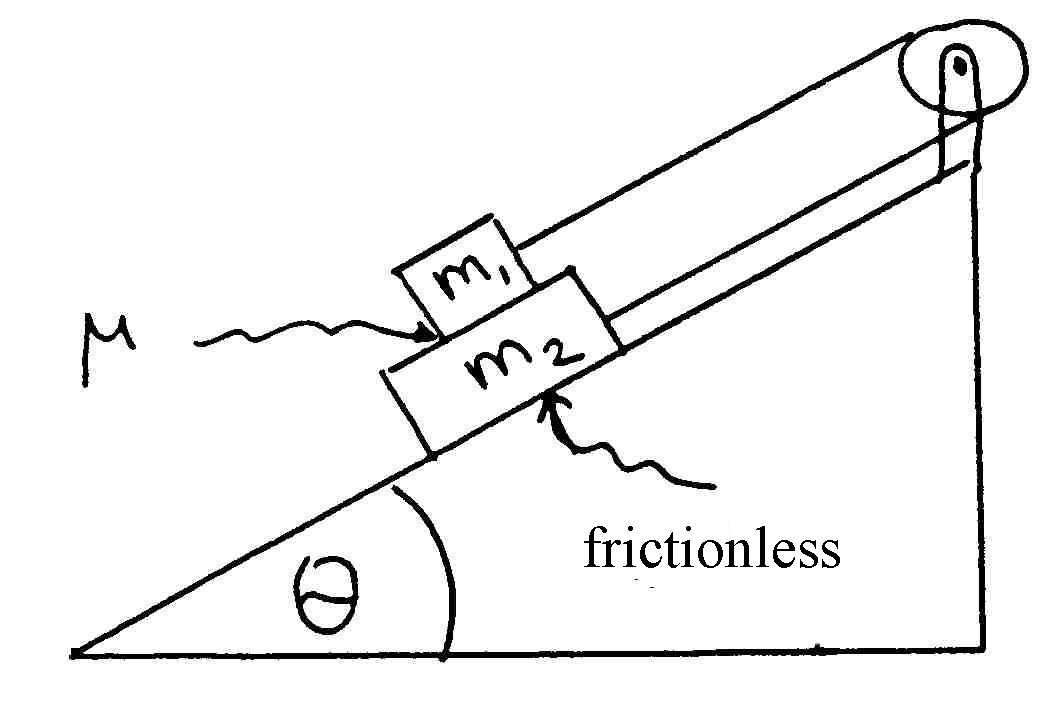
\includegraphics[scale=1.0]{Graphics/h3p8}
\end{center}

What are the magnitudes of the acceleration of the two blocks? Express your answer in terms of $g$, $\mu$, $m_1$, $m_2$, and $\theta$.''

Since $m_2$ is much greater than $m_1$, $m_2$ will slide downhill and $m_1$ uphill... until they slide off each other, that is. The only other possibility is that $a = 0$ and that the system is in equilibrium, because the friction is great enough. I will assume the answer is not zero, though!

Drawing a free-body diagram (a must for most of these questions, but especially this one), we find a lot of forces.\\
As usual, I chose a coordinate system with $x$ parallel to the incline, and $y$ perpendicular. $+x$ is downhill, for no reason in particular.

On block $m_1$, there is friction, gravity/normal force (gravity in 2 dimensions) and tension. On block $m_2$, there is also gravity in two dimensions and a normal force, but we don't need to pay much attention to the $y$ forces, since there is no friction on the ramp. We know that the normal force will cancel gravity, but that's about it for its usefulness. In addition to those, there's tension and a third law reaction force for the friction.

Let's try to write Newton's second law equations in the $x$ direction. I will add up downhill forces, subtract uphill forces, and set it all equal to the mass times acceleration:

\begin{align}
m_1 g \sin \theta + \mu m_1 g \cos \theta - T = - m_1 a\\
m_2 g \sin \theta - T - \mu m_1 g \cos \theta = m_2 a
\end{align}

Not very pretty, is it? I will admit, it took me a few tries to get it right; I first forgot about the third law reaction force for the friction (there's a frictional force uphill on the second block!).\\
As for directions, the first equation has $-m_1 a$ since the acceleration is positive downhill, but the motion will surely be uphill. The second equation has it without the minus sign, since that block will indeed move downhill.

Let's try to solve this by addition; that is, add the left sides to a new left side, and the two right sides to a new right side. The friction should cancel, so finding $a$ should be less painful than by substitution.

\begin{align}
m_1 g \sin \theta + \mu m_1 g \cos \theta - T + m_2 g \sin \theta - T - \mu m_1 g \cos \theta = - m_1 a + m_2 a\\
m_1 g \sin \theta - 2T + m_2 g \sin \theta  = - m_1 a + m_2 a\\
g \sin \theta(m_1 + m_2) - 2T = a(m_2 - m_1)\\
a = \frac{g \sin \theta(m_1 + m_2) - 2T}{m_2 - m_1}
\end{align}

Unfortunately, that doesn't quite get us all the way; we don't know $T$! Let's solve for it from, say, the second equation (either should work, and they're equally complex, so I just picked one). I suppose we'll do substitution after all:

\begin{align}
T &= m_2 g \sin \theta - \mu m_1 g \cos \theta - m_2 a\\
T &= g(m_2 \sin \theta - \mu m_1 \cos \theta) - m_2 a
\end{align}

Combining the two, we get... this monstrosity, which we need to solve for $a$ again:

\begin{align}
a &= \frac{g \sin \theta(m_1 + m_2) - 2(g m_2 \sin \theta - g \mu m_1 \cos \theta - m_2 a)}{m_2 - m_1}\\
a &= \frac{g \sin \theta(m_1 + m_2) - 2g m_2 \sin \theta + 2 g \mu m_1 \cos \theta + 2 m_2 a}{m_2 - m_1}\\
a &= \frac{g \sin \theta(m_1 + m_2) - 2g m_2 \sin \theta + 2 g \mu m_1 \cos \theta}{m_2 - m_1} + \frac{2 m_2 a}{m_2 - m_1}\\
a\left(1 - \frac{2 m_2}{m_2 - m_1}\right) &= \frac{g \sin \theta(m_1 + m_2) - 2g m_2 \sin \theta + 2 g \mu m_1 \cos \theta}{m_2 - m_1}\\
a &= \frac{g \sin \theta(m_1 + m_2) - 2g m_2 \sin \theta + 2 g \mu m_1 \cos \theta}{m_2 - m_1} \cdot \frac{1}{1 - \frac{2 m_2}{m_2 - m_1}}
\end{align}

Goodness, I could use Mathematica to simplify that, but it is accepted as correct!

For the sake of readability, here's a simplified version:

\begin{equation}
a = \frac{g(\sin \theta(m_2 - m_1)) - 2 g m_1 \mu \cos\theta}{m_1 + m_2}
\end{equation}

\section{Problem 9: Conical pendulum}

``A conical pendulum is constructed from a rope of length $\ell$ and negligible mass, which is suspended from a fixed pivot attached to the ceiling. A small ball of mass $m$ is attached to the lower end of the rope. The ball moves in a circle with constant speed in the horizontal plane, while the rope makes an angle $\beta$ with respect to the vertical, as shown in the diagram.

\begin{center}
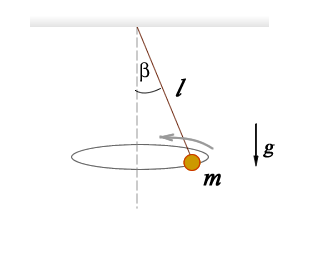
\includegraphics[scale=1.0]{Graphics/h3p9}
\end{center}

(a) Find the tension $F_T$ in the rope. Express your answer in terms of $g$, $m$, $\ell$, and $\beta$.\\
(b) Find the period of the motion (how long does it take the ball to make one circle in the horizontal plane). Express your answer in terms of $g$, $m$, $\ell$, and $\beta$.''

Okay, so let's see. The mass moves in a circle at constant speed: uniform circular motion. We don't know $\omega$ or $T$, though, as that's what we are looking for. We do know the angle and the rope's length, so we should be able to calculate the radius of the (horizontal) circle traced out by the mass itself, however.

In fact, if we forget about the third dimension, we have a very simple right triangle formed by the rope and the axes. We can see that

\begin{align}
\sin \beta &= \frac{r}{\ell}\\
r &= \ell \sin \beta
\end{align}

I will use cylindrical coordinates for this problem; that is, $\hat{r}$ is radially outwards, $\hat{\theta}$ is tangential to the traced out circle (positive counterclockwise, as the motion is), and $\hat{z}$ is upwards.

There is a centripetal acceleration 

\begin{align}
a_c &= \omega^2 (-\vec{r})\\
      &= \omega^2 \ell \sin \beta (-\hat{r})\\
      &= \frac{4 \pi^2}{T^2} \ell \sin \beta (-\hat{r})
\end{align}

towards the center of the traced circle, caused by a centripetal force $m$ times the above.

What other forces are there? Well, there's certainly gravity, $-m g$ if we call upwards $+z$. There's the tension in the string, $F_T$ ($T$ is used for the period) which consists of $z$ and $r$ components. Let's decompose the tension.

\begin{align}
F_{Tz} = F_T \cos \beta\\
F_{Tr} = F_T \sin \beta
\end{align}

The centripetal force is purely in the $-\hat{r}$ direction, so we don't need to decompose that. Neither do we need to decompose gravity, which is purely in the $-\hat{z}$ direction.

The net force on the mass must be the centripetal force, or there wouldn't be \emph{uniform} circular motion. The $z$ component of the tension must cancel out gravity, too, or the mass wouldn't move in a horizontal plane, as it does.\\
Time for Newton's second law. Let's just gather a list of the forces first, so there's no confusion while writing the equations. In the $r$ axis, we have the centripetal force $F_r = a_c m$ inward, and the string tension also inward. In other words, the string tension \emph{provides} (or \emph{is}, essentially) the centripetal force, and thus the cause of the centripetal acceleration.\\
In the $z$ axis, there is gravity downwards, and a tension component upwards, which must cancel out to yield zero net force.\\
Lastly, in addition to $F_r = a_c m$, we can say that $a_c = \omega^2 r$, and we derived an expression involving the period earlier, so we find, for the $r$ and $z$ axes respectively,

\begin{align}
a_c m = F_T \sin \beta \Rightarrow \frac{4\pi^2}{T^2} \ell m \sin (\beta) &= F_T \sin \beta\\
m g &= F_T \cos \beta
\end{align}

And we now at the point where we have two equations with two unknowns. I'll try to solve them manually. Solving the second for $F_T$ is easy:

\begin{equation}
F_T = \frac{m g}{\cos \beta}
\end{equation}

A-ha, nice! It's already in terms of $g$, $m$ and $\beta$, so that's the finished answer for part (a)! Now, let's substitute that into the other one and solve for the period $T$, which was surprisingly easy:

\begin{align}
\frac{4\pi^2}{T^2} \ell m \sin (\beta) &= \frac{m g}{\cos \beta} \sin \beta\\
\frac{4\pi^2}{T^2} \ell m &= \frac{m g}{\cos \beta}\\
\frac{2 \pi \sqrt{\ell cos \beta}}{\sqrt{g}} &= T
\end{align}

Tension cannot be negative, so we ignore the second solution.

\section{Problem 10: Stacked blocks 2}

``A block of mass $m_B = \SI{15}{kg}$ is on top of a long slab of mass $m_S = \SI{9}{kg}$, and the slab is on top of a horizontal table as shown. A horizontal force of magnitude $F = \SI{294}{N}$ is applied on the block. As a result the block moves relative to the slab and the slab moves relative to the table. There is friction between all surfaces. The coefficient of kinetic friction between the block and the slab is $\mu_1 = 0.7$, and the coefficient of kinetic friction between the slab and the table is $\mu_2 = 0.1$. Take $g$ to be $\SI{9.81}{m/s^2}$, and enter your answer to 3 significant figures.

\begin{center}
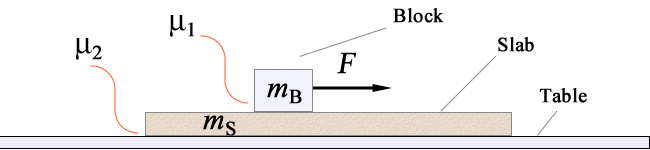
\includegraphics[scale=1.0]{Graphics/h3p10}
\end{center}

(a) What is the magnitude of the block's acceleration?\\
(b) What is the magnitude of the slab's acceleration?''

I guessed they saved the best for last! I was expecting to see something like this (friction in two places) on the exam, but not quite on the homework.

Ah well, let's get to it. The free-body diagram comes first, as always. Lots of forces; let's start with the vertical ones, since the frictional forces depend on the normal forces.\\
The block and a slab each have a gravitational force downwards, and a normal force upwards; I'll denote these by $N_B$ for the normal force \emph{on} the block (by the slab), and $N_S$ for the normal force on the slab (by the table):

\begin{align}
N_B &= m_B g\\
N_S &= g(m_B + m_S)
\end{align}

This then gives us the frictional forces $F_{F1}$ (friction that limits the block's movement) and $F_{F2}$ (friction that limits the slab's movement), named after the friction coefficients in the problem description:

\begin{align}
F_{F1} &= \mu_1 m_B g\\
F_{F2} &= \mu_2 g(m_B + m_S)
\end{align}

What is the direction of these forces? Some books appear to write this badly, but here's a quote from \cite[p.~123]{serway}:

\begin{quote}
Sometimes, an incorrect statement about the friction force between an object and a surface is made -- ``the friction force on an object is opposite to its motion or impending motion'' -- rather than the correct phrasing, ``the friction force on an object is opposite to its motion or impending motion \emph{relative to the surface}.''
\end{quote}

So in other words, since the slab moves to the right relative to the table, the friction force there is to the left.\\
The block should also move right relative to the slab (how could the slab possibly accelerate \emph{faster}?), so that frictional force should also be to the left.

Do we now have all the forces? We have covered the $y$ axis with gravitational forces and normal forces, and friction on all surfaces. Left are the third law reaction forces due to friction.

Because there is a frictional force $F_{F1}$ by the slab (middle) on the block (top), there must be a force of equal magnitude in the opposite direction on the slab, so we have a rightwards force $F_{F1}$ on the slab that we must not forget about.\\
There is also a leftwards frictional force on the slab from the table, so there is a reaction force there too, but since it's on the table, which we take to be immovable, we can ignore that force.

All in all we have, ignoring vertical forces, on the block: the external force $F$ to the right, friction $F_{F1}$ to the left.\\
On the slab, we have a reaction force $F_{F1}$ to the \emph{right}, and ``regular'' friction with the table $F_{F2}$ towards the left.

Let's also not forget that they don't accelerate together; the forces add up to some $m_B a_B$ and $m_S a_S$, but we can't solve for a combined $a$.

We can finally start writing second law equations, and substituting in the actual values. I will take $+x$ to be towards the right. First the block, then the slab:

\begin{align}
F - F_{F1} = m_B a_B &\Rightarrow F - \mu_1 m_B g = m_B a_B\\
F_{F1} - F_{F2} = m_S a_S &\Rightarrow \mu_1 m_B g - \mu_2 g(m_B + m_S) = m_S a_S
\end{align}

Two equations, two unknowns (the accelerations), how unusual! However, they don't depend on each other at all, so this should be simple! Let's solve them one at a time:

\begin{align}
F - \mu_1 m_B g = m_B a_B\\
a_B = \frac{F - \mu_1 m_B g}{m_B} \approx \SI{12.733}{m/s^2}
\end{align}

\begin{align}
\mu_1 m_B g - \mu_2 g(m_B + m_S) = m_S a_S\\
a_S = \frac{\mu_1 m_B g - \mu_2 g(m_B + m_S)}{m_S} \approx \SI{8.829}{m/s^2}
\end{align}

Nice!

\end{document}